%TODO, before release, do spell-check

\documentclass[a4paper, 11pt]{article} % Font size (can be 10pt, 11pt or 12pt) and paper size (remove a4paper for US letter paper)

\usepackage[protrusion=true,expansion=true]{microtype} % Better typography
\usepackage{graphicx} % Required for including pictures
\usepackage{hyperref}
\usepackage{float}

\usepackage{mathpazo} % Use the Palatino font
\usepackage[T1]{fontenc} % Required for accented characters
\linespread{1.05} % Change line spacing here, Palatino benefits from a slight increase by default
\usepackage[british]{babel}

\makeatletter
\renewcommand\@biblabel[1]{\textbf{#1.}} % Change the square brackets for each bibliography item from '[1]' to '1.'
\renewcommand{\@listI}{\itemsep=0pt} % Reduce the space between items in the itemize and enumerate environments and the bibliography

\renewcommand{\maketitle}{ % Customize the title - do not edit title and author name here, see the TITLE block below
\begin{flushright} % Right align
{\LARGE\@title} % Increase the font size of the title

\vspace{50pt} % Some vertical space between the title and author name

{\large\@author} % Author name
\\\@date % Date

\vspace{40pt} % Some vertical space between the author block and abstract
\end{flushright}
}

%----------------------------------------------------------------------------------------
%	TITLE
%----------------------------------------------------------------------------------------

\title{\textbf{PhyloGeoTool}\\ % Title
User Manual} % Subtitle

\author{\textsc{Ewout Vanden Eynden, Pieter Libin, Kristof Theys, Guy Baele} % Author
\\{\textit{Rega Institute for Medical Research, KU Leuven}}} % Institution

\date{\today} % Dates

%----------------------------------------------------------------------------------------

\hyphenation{Phylo-Geo-Tool}

\begin{document}
\maketitle % Print the title section

%TODO update images (when everything is final)

\vspace{30pt} % Some vertical space between the abstract and first section

%------------------------------------------------
\tableofcontents
\newpage

This document explains how to use the PhyloGeoTool software. PhyloGeoTool is a web application that is installed on a web server, and can be accessed via a web browser. 
Most users will access a publicly accessible instance of the PhyloGeoTool (i.e. an instance that was already deployed on a web server). 
An example of a publicly available instance of the PhyloGeoTool that allows to explore a large HIV cohort (i.e. EuResist \cite{Zazzi2012}) can be found at \url{http://phylogeotool.gbiomed.kuleuven.be/euresist/}.
It is however also possible to install your own instance of the PhyloGeoTool; for this, we refer to the installation manual \footnote{(TODO (Ewout): add link)}. Such an instance can be used to investigate a dataset on a local computer or to host your own public PhyloGeoTool instance.


\section{Getting started}

PhyloGeoTool implements a visual method to explore large phylogenetic trees and to depict characteristics of strains and clades, including their geographic context, in an interactive way.
The tool also provides the possibility to insert new virus strains into the existing phylogenetic tree, allowing users to gain insight in the placement of such new strains without the need to reconstruct the phylogeny.

A particular PhyloGeoTool instance can be used by navigating the browser to the URL at which this instance has been deployed. For example, the aforementioned public EuResist instance of the PhyloGeoTool is deployed at \url{http://phylogeotool.gbiomed.kuleuven.be/euresist/}, and thus, you should navigate your browser to this exact URL
\footnote{TODO (KT): explaining what instances are all about, is easier if you can mention more than 1 instance. 
Perhaps Lize will have a HCV/DENV instance ready soon, that we can add here, but maybe we should both deploy the EuResist and PT tool, such that we can list them in this section.}.
Note that any browser (Chrome, Firefox, Internet Explorer) should do.\\

\noindent If you experience any problems, please contact us phylogeotool@kuleuven.be.


\section{Core functionality and user interface}
\label{sec:core_func_user_interface}
%TODO (Ewout): update all images when the software is ready
%TODO (Ewout): all images are 400x400px, why not use a percentage, and let the images be their natural dimenions?
\begin{figure}[H]
\centering
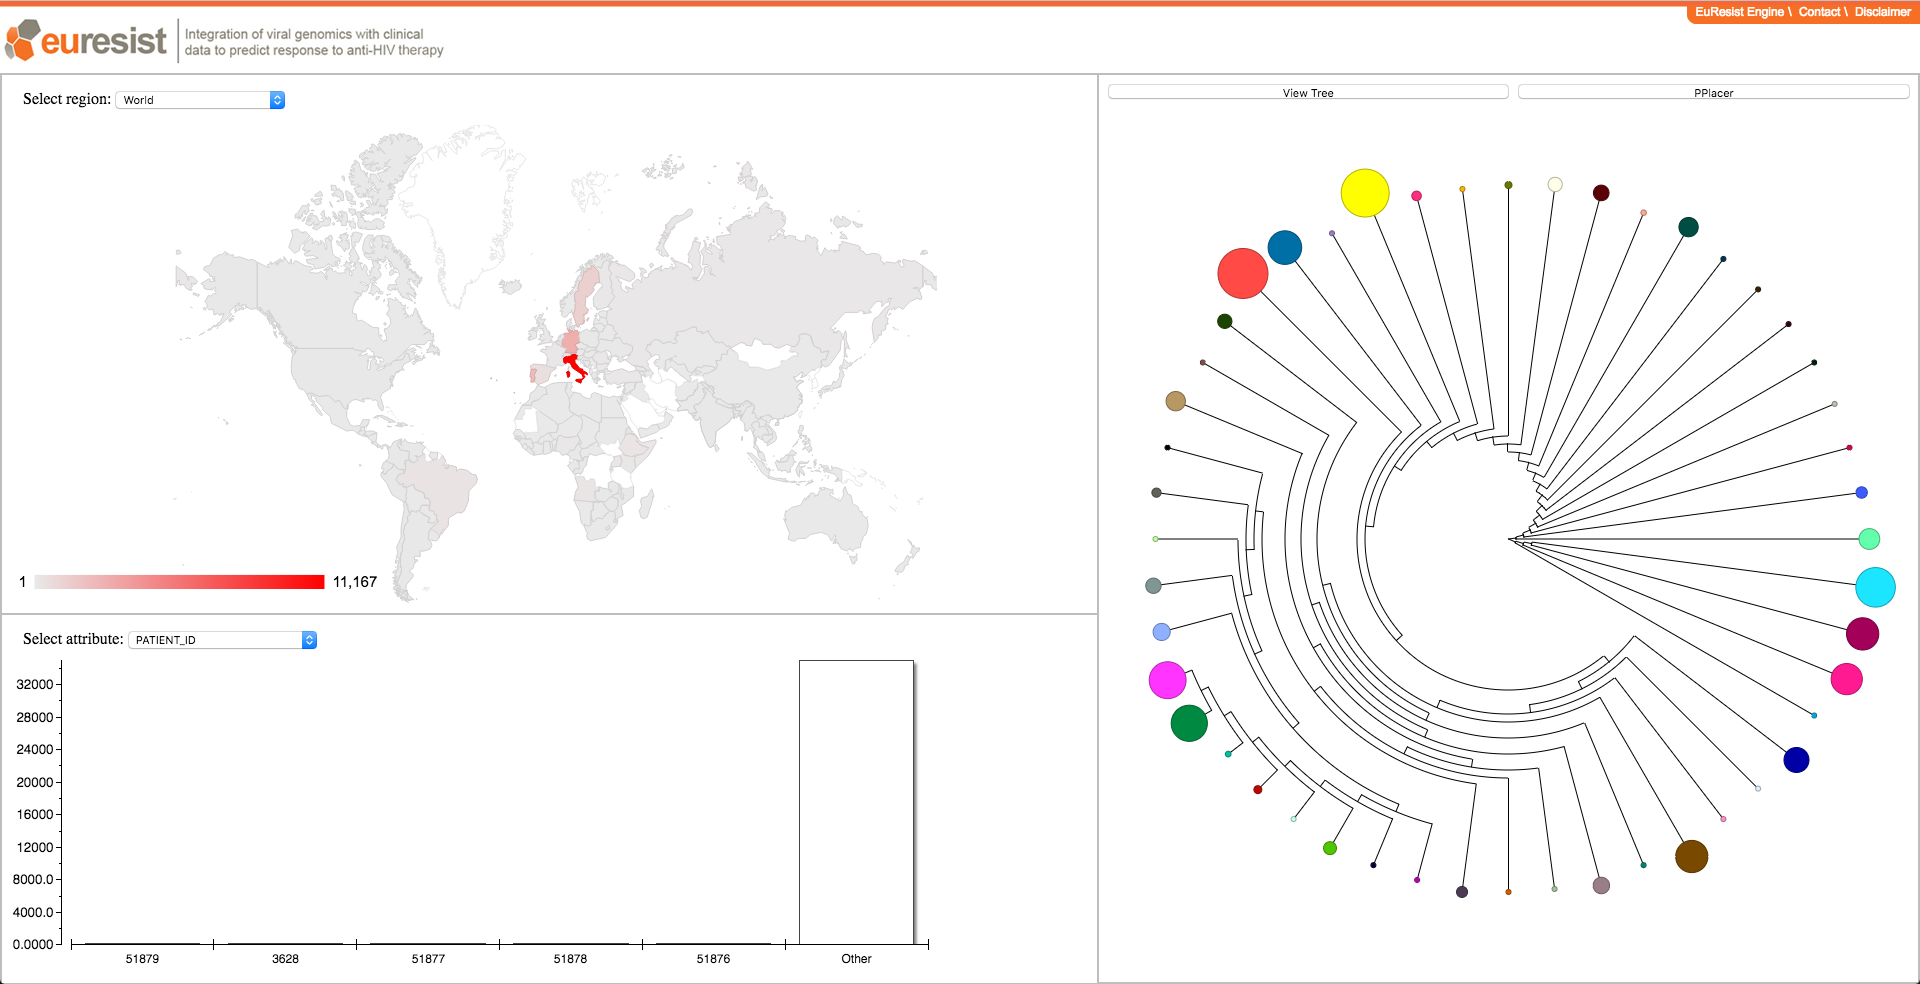
\includegraphics[scale=0.1875]{images/defaultScreenshot.png}
\vspace{-0.75cm}
\caption{Start and main view of the PhyloGeoTool. 
  The panel on the upper left shows a map that depicts the geographical distribution of the sequences of the partitioned phylogeny; the lower left panel shows a bar chart that depicts the value distribution for one of the sequence attributes; and the right panel shows a top-level view of the clustering of the tree, as determined by our clustering algorithm (TODO (Ewout): add reference to our paper as a footnote) .}
\label{fig:initialview}
\end{figure}

The PhyloGeoTool is divided into different panels (see Figure \ref{fig:initialview}): 
\begin{itemize}
  \item The top left panel shows a map where each country is colored according to a gradient, where a darker color signifies that more sequences are originating from this country. 
    A drop-down box allows you to select the geographic region on which you want to focus (e.g. Europe, North America, \ldots).
  \item The right panel shows a top-level view of the clustering of the tree (initially the root of the tree), as determined by our clustering algorithm. (TODO: GB: need to say where the readers can find our clustering algorithm, see footnote above, to be made by ewout)
  A button allows you to visualise the phylogenetic tree in its entirety, colored according to the shown clusters.
  \item The bottom left panel shows a histogram or bar chart depending on the chosen attribute. If the attribute is represented by a continuous dataset, a histogram will be shown while a discrete dataset is displayed by a bar chart plot.
  The histogram or bar chart shows a certain attribute (i.e. characteristic) from all sequences currently visualized in the tree panel on the right. 
  A drop-down box allows you to select the attribute to be plotted on the bar chart. 
  The attributes available for selection depend on the attributes made available by the PhyloGeoTool instance.
\end{itemize}


\subsection{Hovering and clicking cluster nodes}
\begin{figure}[H]
\centering
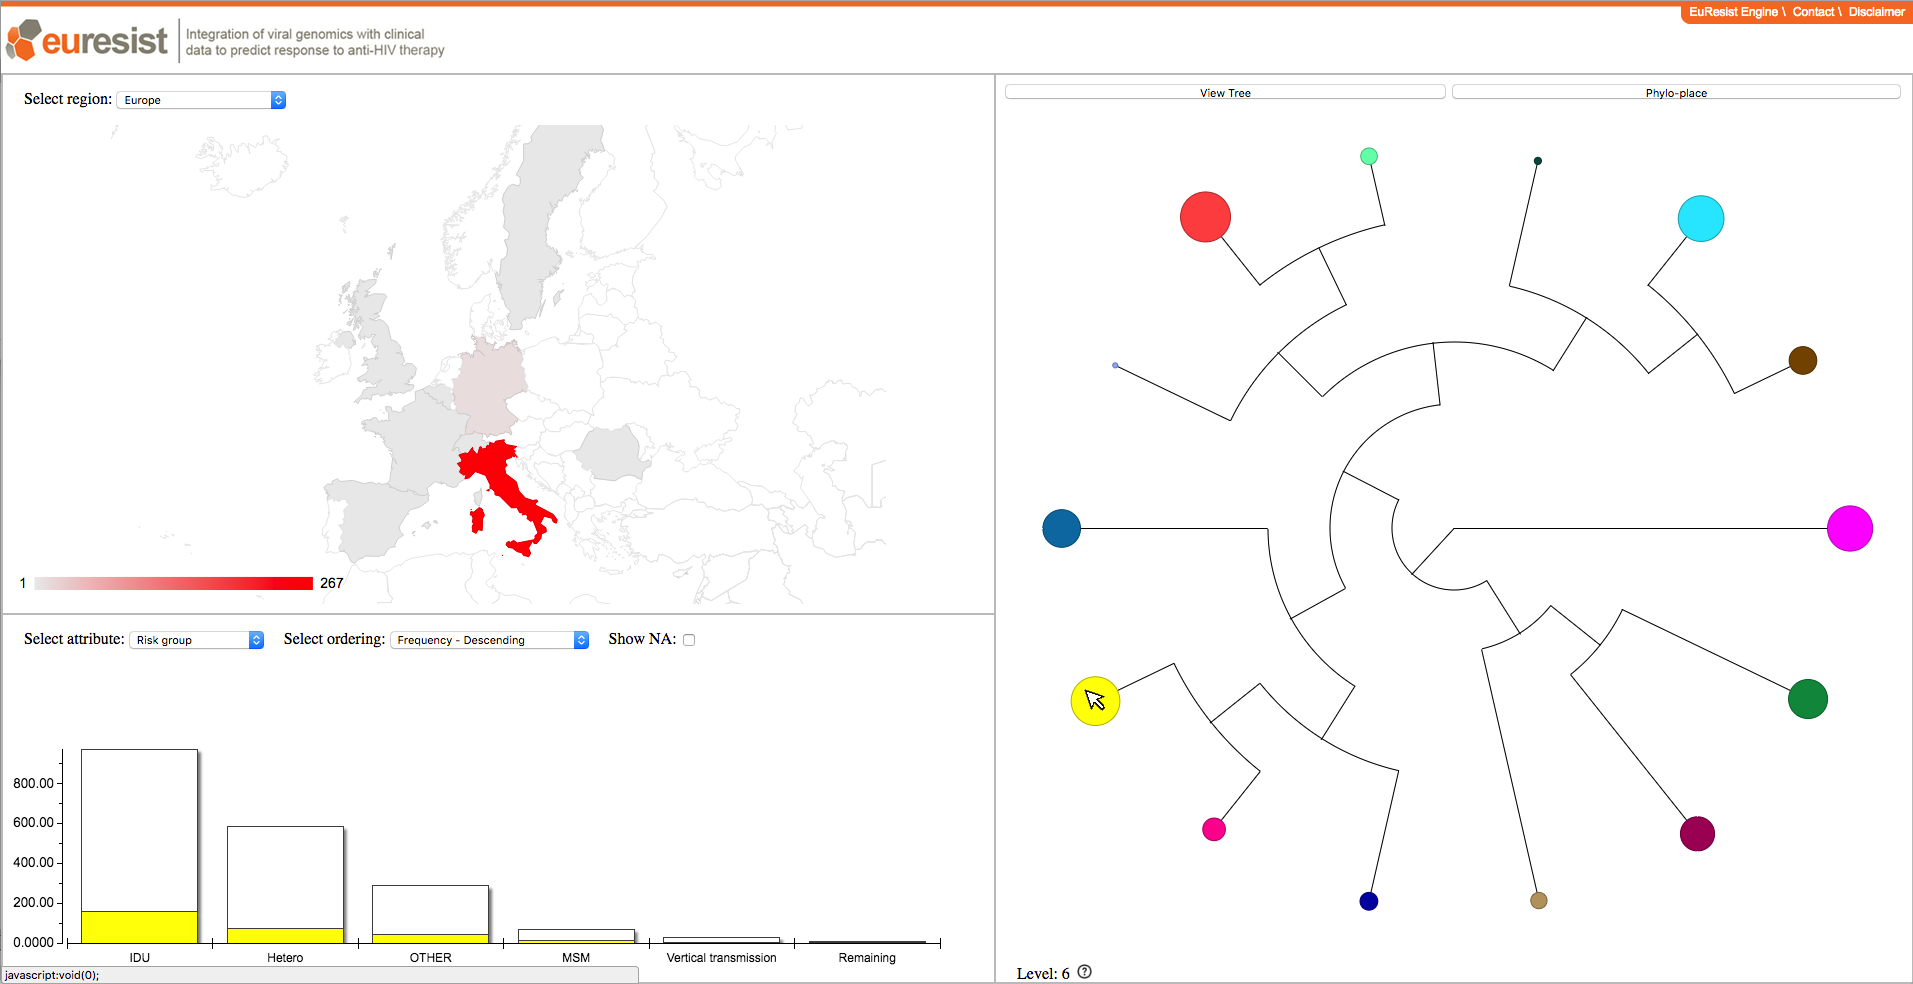
\includegraphics[scale=0.1875]{images/hover_node.PNG}
\vspace{-0.75cm}
\caption{Hovering over a node in the cluster phylogeny.}
\label{fig:hovernode}
\end{figure}

When the user hovers the mouse (TODO (GB): mouse pointer?) over a node in the clustered phylogeny, both the attribute chart and the map are updated. 
The attribute chart will be extended (i.e. extra bars will be shown on top of the original chart for each value) with the data that is located in the cluster over which the mouse (TODO (GB): mouse pointer?) hovers. (TODO: GB: extended, maybe overlaid?)
The map, on the other hand, will only show the geographic distribution of the sequences found in the cluster over which the mouse (TODO (GB): mouse pointer?) hovers.

When you click on a node in the clustered phylogenetic tree, the PhyloGeoTool will navigate to the clustering of this particular node (i.e. will go down one level in the node on the clustered phylogenetic tree).
A counter on the bottom left of the cluster panel keeps track of the depth of the navigation. 
As you can visit a cluster node by clicking it, you can go back to into your navigational path by using the browser's 'Back' button.
The depth of the navigation is also shown when you hover over the '?' which is shown next to 'Level: '. (TODO(KT): say something about going back to the root ot the tree)

Additionally, the URL encodes the level of descent in the clustered phylogenetic tree. 
A URL can hence be bookmarked or shared to go back at the exact location in the clustered phylogenetic tree. 


\subsection{Select a geographic region}
\begin{figure}[H]
\centering
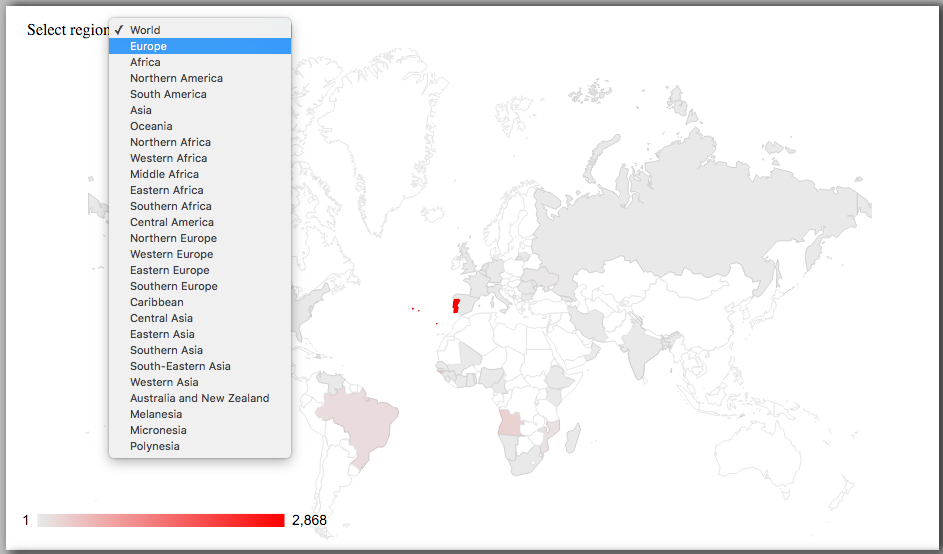
\includegraphics[scale=0.38]{images/change_country.PNG}
\vspace{-0.75cm}
\caption{Change the region in the drop down box}
\label{fig:change_region}
\end{figure}
You can select your geographical region of interest in the drop-down box on top of the map (see Figure \ref{fig:change_region}). 


\subsection{Select a sequence attribute}
\begin{figure}[H]
\centering
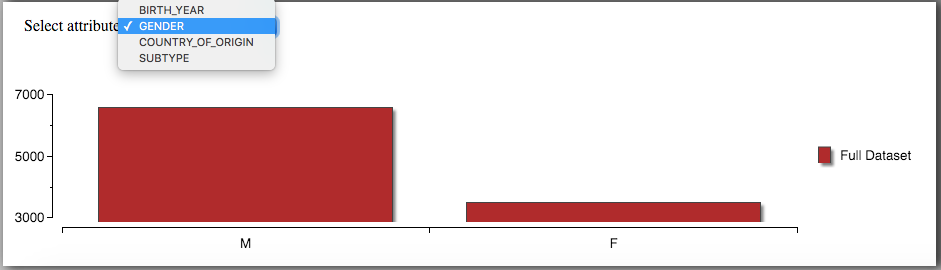
\includegraphics[scale=0.38]{images/change_attr.PNG}
\vspace{-0.75cm}
\caption{Change the attribute in the drop down box}
\label{fig:change_attr}
\end{figure}
You can select an attribute of interest in the drop-down box on top of the attribute chart (see Figure \ref{fig:change_attr}).


\subsection{Export the phylogenetic tree}
\begin{figure}[H]
\centering
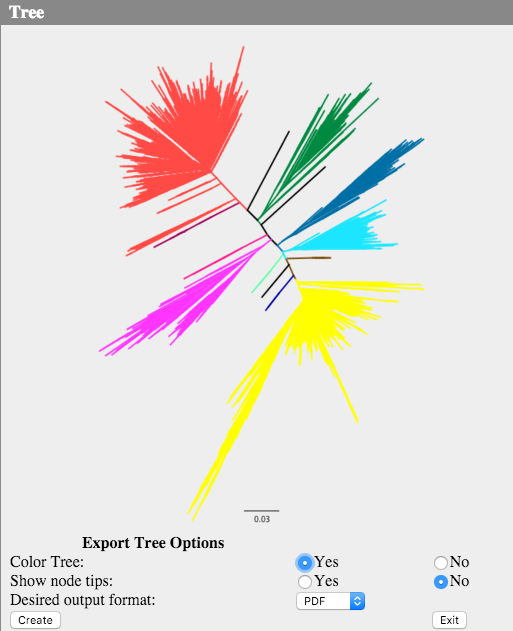
\includegraphics[scale=0.50]{images/view_tree.PNG}
\vspace{-0.25cm}
\caption{Visualising the phylogenetic tree, colored according to the clustering scheme.}
\label{fig:view_tree}
\end{figure}


\begin{figure}[H]
\centering
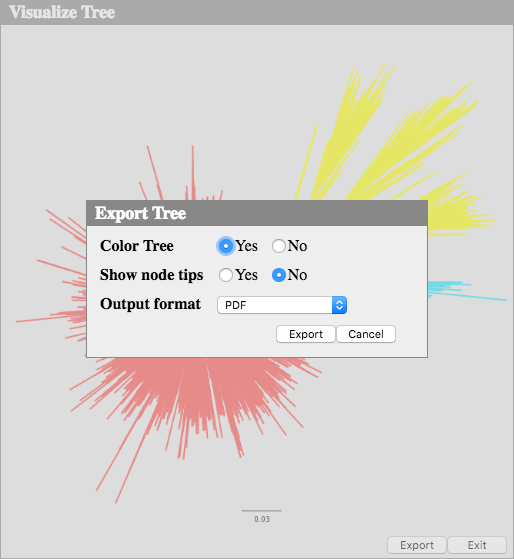
\includegraphics[scale=0.50]{images/export_tree.PNG}
\vspace{-0.25cm}
\caption{Form displaying the preferred settings to export the shown phylogenetic tree.}
\label{fig:export_tree}
\end{figure}

When the 'View Tree' button (located at the top of the clustered phylogeny panel) is clicked, a pop-up window is shown (Figure \ref{fig:view_tree}) that visualizes the phylogeny as a radial phylogenetic tree. 
The colours in the radial tree correspond to the colors of the clusters.

(TODO PL, you alternate between American and British English in the document; do you prefer 'color' or 'colour'?, will check with a spell checker and use British)
\break
\break
On the bottom of the popup window, there are two buttons: 'Export' and 'Exit'.
The button with label 'Export' will show a window similar to the one shown in Figure \ref{fig:export_tree}. There are three options available that allows the customization of the export:
\begin{itemize}
\item Color Tree: enable/disable the coloring of tree based on the clusters' color.

\item Show node tips: include/ecxclude leaf names in the phylogenetic tree.
\item Output Format: the format in which you want your tree to be downloaded (i.e. PDF, NEXUS, SVG, PNG).
\end{itemize}
  

\footnote{Exports in the NEXUS file format can be visualized in programs such as FigTree (\url{http://tree.bio.ed.ac.uk/software/figtree/}).}  

\subsection{Automated phylogenetic placement of sequences}
Phylogenetic placement enables the placement of unknown query sequences onto an existing phylogenetic tree, without the need to re-compute the entire phylogeny (which is a time-consuming process, especially when a large number of sequences is involved). 
In the PhyloGeoTool, we use phylogenetic placement to position new sequences onto the phylogeny, in a reasonable amount of time (i.e. minutes). 
We implement this placement using the well-known pplacer software package \cite{Matsen2010}.

To place your sequences on the cluster phylogeny, click the 'Phylo-place' button (TODO (PL) update button name) in the clustering window. 
A window (see Figure \ref{fig:pplacerwindow}) will pop up that enables you to place your sequences. 

\begin{figure}[H]
\centering
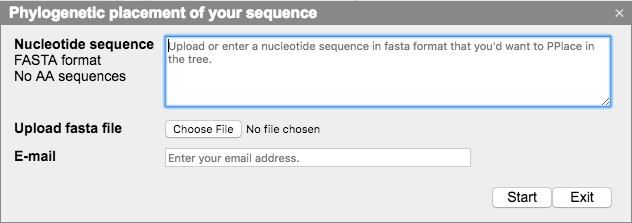
\includegraphics[scale=0.50]{images/pplacerWindow.png}
\vspace{-0.25cm}
\caption{Phylogenetic placement window.}
\label{fig:pplacerwindow}
\end{figure}

\noindent There are two ways to add a new sequence to the tree:
\begin{itemize}
\item Paste your sequence in the 'Nucleotide sequence' field.
\item Upload a FASTA file containing the nucleotide sequence using the file chooser.
\end{itemize}
Currently, we only support the submission of 1 sequence at a time.
If you submit more than 1 sequence to be added to the phylogenetic tree, a warning will be shown.

Once the Pplacer process finished you will receive an e-mail with a link to show the placement result.
You will be taken to the original PhyloGeoTool webpage (such as described in Section \ref{sec:core_func_user_interface}) with this difference that the cluster, which contains the pplaced sequence, is surrounded by a dashed line (see Figure \ref{fig:pplacer-view}). 

\begin{figure}[H]
\centering
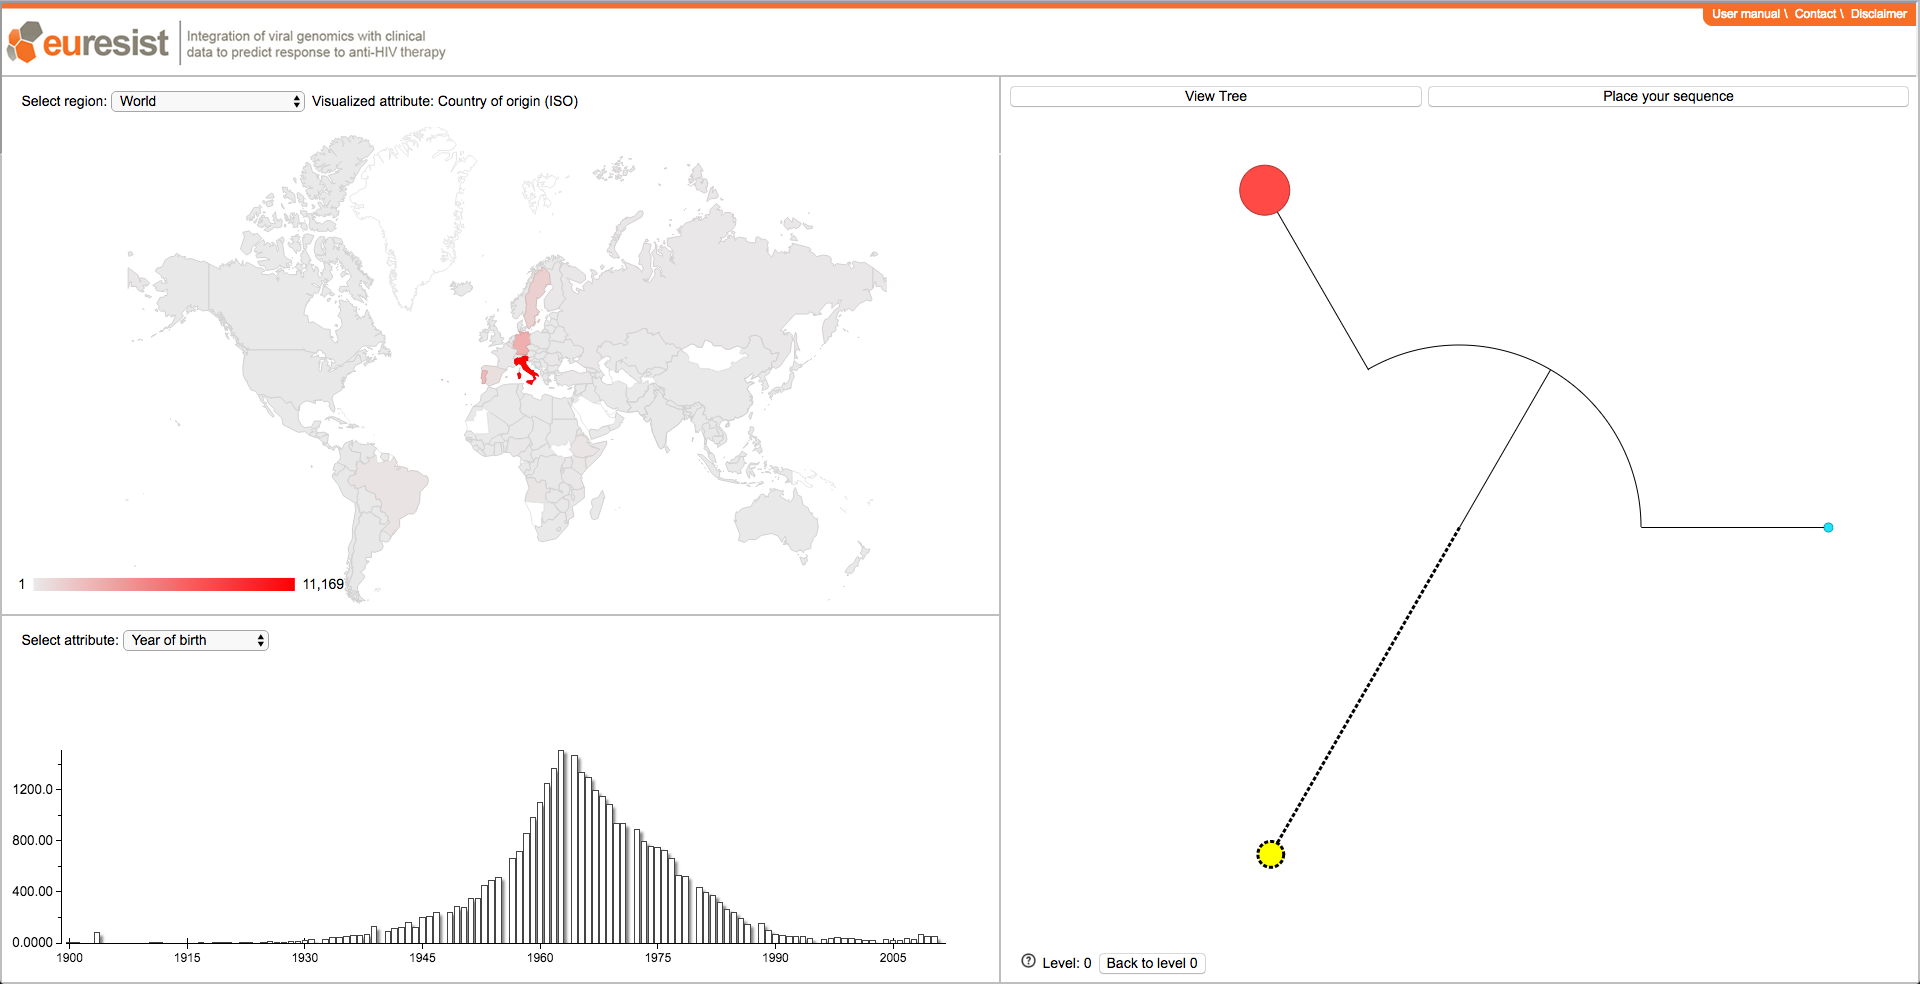
\includegraphics[scale=0.1875]{images/pplaced_sequence.png}
\vspace{-0.75cm}
\caption{Start and main view of the PhyloGeoTool with a Pplaced sequence.}
\label{fig:pplacer-view}
\end{figure}

%After submission: make video
%\section{Example: exploring a large HIV-1 dataset}

%As mentioned earler, we host a publicly available instance of the PhyloGeoTool that uses all HIV-1 data that is currently available in the EuResist Integrated Data Base \cite{Zazzi2012}. 
%This database contains virus genotypes, clinical responses and epidemiological markers of more than 66.000 patients from 12 different countries.
%We made a YouTube video available where all features we discussed earlier are demonstrated using the EuResist PhyloGeoTool instance: \footnote{(TODO: add video)}.

%TODO (when everything is ready): Video scenario:\\
% as in this video (that we created earlier, for a presentation I gave in June) -> \url{https://drive.google.com/open?id=0B-0JA80u3ZPTbVVTNThrVXVRam8} \\
% with these additions/changes :\\  
% - we should talk during the video \\
%- we should do an export in NEXUS format and open this in FigTree \\
% - when phylo-placing, go down to the level where the placement was done\\
% - when phylo-placing, I don't think it is necessary to show the upload, simply pasting the sequence in the field is OK \\



\section{Contact Information and support }
% once published: write something like 
% Please cite ....

The PhyloGeoTool is developed and maintained by the Rega Institute KU Leuven.
You can contact us on \href{mailto:phylogeotool@kuleuven.be}{phylogeotool@kuleuven.be}



\bibliographystyle{plain}
\bibliography{References}

\end{document}
